\documentclass{article}
\usepackage[utf8]{inputenc}

\usepackage{calrsfs}
\usepackage{natbib}
\usepackage{graphicx}
\usepackage{mathtools}
\usepackage{amsmath}
\usepackage{braket}
\usepackage{amssymb}
\usepackage[makeroom]{cancel}



\title{Master}
\author{Juan Carlos Linares Rugeles}
\date{February 2018}

\begin{document}

\maketitle

\section{Riboswitch}

\begin{figure}[h!]
\centering
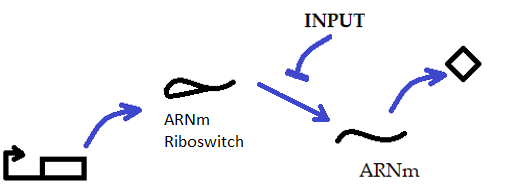
\includegraphics[scale=1]{Riboswitch}
\caption{Riboswitch system scheme.}
\label{fig:estructura}
\end{figure}

\begin{align*}
    T &\xrightarrow[]{\big{K_T}} T+1       & P &\xrightarrow[]{\big{K_PT}} P+1         & R &\xrightarrow[]{\big{\mu_+ET}} R+1          \\
    T &\xrightarrow[]{\big{\mu_-R}} T+1    & P &\xrightarrow[]{\big{\gamma_PP}} P-1    & R &\xrightarrow[]{\big{(\gamma_R + \mu_-)R}} R-1 \\
    T &\xrightarrow[]{\big{\gamma_TT}} T-1 &\\                                    
    T &\xrightarrow[]{\big{\mu_+ET}} T-1   &\\ 
\end{align*}

\subsubsection{ Langevin equations}

Langevin equations derived for this system without the noise term.

\begin{align}
    \frac{d}{dt}T &= K_T + \mu_-R - \mu_+ET - \gamma_TT \\
    \frac{d}{dt}P &= K_PT - \gamma_PP \\
    \frac{d}{dt}R &= \mu_+ET - (\gamma_R + \mu_+)R 
\end{align}

\subsection{ Master equation}

Equation that describes the probability change over time, determined by the amount of particles in a certain state $(T, P, R)$. Here the state is not always specified entirely. For example: $P(T-1)$ refers to the state $(T, P, R)$ in which only the variable $T$ is changed by $-1$; $P(T-1)=P(T-1, P, R)$.

\begin{align*}
    \frac{d}{dt}P(T,P,R) &= K_TP(T-1) - K_TP(T) + \gamma_T(T+1)P(T+1) - \gamma_TTP(T) \\
                         &+ \mu_+E(T+1)P(T+1,R-1) - \mu_+ETP(T,R) \\
                         &+ \mu_-(R+1)P(T-1,R+1) - \mu_-RP(T,R)\\
                         &+ \gamma_R(R+1)P(R+1) - \gamma_RRP(R) + K_PTP(P-1) - K_PTP(P)\\
                         &+ \gamma_P(P+1)P(P+1) - \gamma_PPP(P)
\end{align*}

Defining:

\begin{equation}
    F = \sum_T\sum_P\sum_R X_1^TX_2^PX_3^RP(T,P,R)
\end{equation}


A system of associated variables is obtained:

\begin{align*}
    T & \xrightarrow{F} X_1  &  P &\xrightarrow{F} X_2  &  R &\xrightarrow{F} X_3
\end{align*}

Then, applying the above definition to the master equation, the latter transforms into the moment-generating function of the $P(T,P,R)$ distribution: 

\begin{equation}
    \left.\begin{aligned}
            \frac{d}{dt}F &= K_T(X_1 -1)F - \gamma_T(X_1 - 1)\frac{\partial}{\partial X_1}F\\
                          &+ \mu_+E(X_3 - X_1)\frac{\partial}{\partial X_1}F + \mu_-(X_1 - X_3)\frac{\partial}{\partial X_3}F\\
                          &- \gamma_R(X_3 - 1)\frac{\partial}{\partial X_3}F + K_PX_1(X_2 - 1)\frac{\partial}{\partial X_1}F - \gamma_P(X_2 - 1)\frac{\partial}{\partial X_2}F
            \end{aligned}
    \right\}
    \qquad DF
 \end{equation}
\\*
\\*

Where $D$ is defined as the differential operator that satisfies: $\Dot{F} = DF$. Now, defining $\partial_i = \frac{\partial}{\partial X_i}$, the equations for the moments are generated via derivatives of $F$.

\begin{itemize}
    \item $\partial_1$
\end{itemize}
\begin{align*}
    \partial_1\Dot{F} &= K_TF - \gamma_T\partial_1F - \mu_+E\partial_1F + \mu_-\partial_3F + K_P(X_2-1)\partial_1F + D\partial_1F\\
    \Longrightarrow   & \partial_1\Dot{F}\mid_{x_i=1} = <\Dot{T}> = K_T - (\gamma_T + \mu_+E)<T> + \mu_-<R>
\end{align*}

\begin{itemize}
    \item $\partial_2$
\end{itemize}
\begin{align*}
    \partial_2\Dot{F} &= K_PX_1\partial_1F - \gamma_p\partial_2F + D\partial_2F\\
    \Longrightarrow   & \partial_2\Dot{F}\mid_{x_i=1} = <\Dot{P}> = K_P<T> - \gamma_P<P>
\end{align*}

\begin{itemize}
    \item $\partial_3$
\end{itemize}
\begin{align*}
    \partial_3\Dot{F} &= \mu_+E\partial_1F - \mu_-\partial_3F - \gamma_R\partial_3F + D\partial_3F\\
    \Longrightarrow   &  \partial_3\Dot{F}\mid_{x_i=1} = <\Dot{R}> = \mu_+E<T> - (\mu_- + \gamma_R)<R>
\end{align*}

\begin{itemize}
    \item $\partial_1\partial_1$
\end{itemize}
\begin{align*}
    \partial_1\partial_1\Dot{F} &= K_T\partial_1F - \gamma_T\partial_1\partial_1F - \mu_+E\partial_1\partial_1F + \mu_-\partial_3\partial_1F + K_P(X_2 - 1)\partial_1\partial_1F\\
                                &+ \partial_1D\partial_1F\\
                                &= 2\{K_T\partial_1F - \gamma_T\partial_1\partial_1F - \mu_+E\partial_1\partial_1F + \mu_-\partial_3\partial_1F + K_P(X_2 - 1)\partial_1\partial_1F\} \\
                                &+ D\partial_1\partial_1F\\
            \Longrightarrow     & \partial_1\partial_1\Dot{F}\mid_{x_i=1} = <\Dot{T(T-1)}> = <\Dot{T^2}> - <\Dot{T}>\\
    <\Dot{T^2}> - <\Dot{T}>     &= 2\{K_T<T> - (\gamma_T + \mu_+E)[<T^2> - <T>] + \mu_-<RT>\}
\end{align*}

\begin{itemize}
    \item $\partial_2\partial_2$
\end{itemize}
\begin{align*}
    \partial_2\partial_2\Dot{F} &= \partial_2\partial_2DF = \partial_2[(\partial_2D)F] + \partial_2[D(\partial_2F)]\\
                                &= (\partial_2^2D)F + (\partial_2D)(\partial_2F) + (\partial_2D)(\partial_2F) + D(\partial_2^2F)\\
                                &= \cancelto{0}{(\partial_2^2D)F} + 2(\partial_2D)(\partial_2F) + D(\partial_2^2F)\\
                                &= 2\{K_PX_1\partial_1\partial_2F - \gamma_P\partial_2\partial_2F\} + D\partial_2\partial_2F\\
            \Longrightarrow     & \partial_2\partial_2\Dot{F}\mid_{x_i=1} = <\Dot{P^2}> - <\Dot{P}> = 2\{K_P<TP> - \gamma_P[<P^2> - <P>]\}
\end{align*}

Since $D$ is linear in $X_1, X_2, X_3$, then $\partial_i^nD=0, \forall n \ge 2, n \in \mathbb{N}$.

\begin{itemize}
    \item $\partial_3\partial_3$
\end{itemize}
\begin{align*}
    \partial_3\partial_3\Dot{F} &= 2( \mu_+E\partial_1\partial_3F - \mu_-\partial_3\partial_3F - \gamma_R\partial_3\partial_3F) + D\partial_3\partial_3F\\
            \Longrightarrow     & \partial_3\partial_3\Dot{F}\mid_{x_i=1} = <\Dot{R^2}> - <\Dot{R}> = 2\{\mu_+R<TR> - (\mu_- + \gamma_R)[<R^2> - <R>]\}
\end{align*}

\begin{itemize}
    \item $\partial_1\partial_2$
\end{itemize}
\begin{align*}
    \partial_2\partial_1\Dot{F} &= K_T\partial_2F - \gamma_T\partial_2\partial_1F - \mu_+E\partial_2\partial_1F + \mu_-\partial_2\partial_3F + K_P\partial_1F + K_P(X_2 - 1)\partial_2\partial_1F  \\
                                &\underbrace{+ K_PX_1\partial_1\partial_1F - \gamma_P\partial_2\partial_1F + D\partial_2\partial_1F}_{\partial_2(D\partial_1F)}\\
    \Longrightarrow & \partial_2\partial_1\Dot{F}\mid_{X_i=1} = <\Dot{PT}> = K_T<P> - \gamma_T<PT> -\mu_+E<PT> + \mu_-<PR>\\
                    & \hspace{100pt}  + K_P<T> + K_P[<T^2> - <T>] - \gamma_P<PT>
\end{align*}

\begin{itemize}
    \item $\partial_1\partial_3$
\end{itemize}
\begin{align*}
    \partial_3\partial_1\Dot{F} &= K_T\partial_3F - \gamma_T\partial_3\partial_1F - \mu_+E\partial_3\partial_1F + \mu_-\partial_3\partial_3F + K_P(X_2 - 1)\partial_3\partial_1F\\
                                &\underbrace{+ \mu_+E\partial_1\partial_1F - \mu_-\partial_3\partial_1F - \gamma_R\partial_3\partial_1F + D\partial_3\partial_1F}_{\partial_3(D\partial_1F)}\\
                \Longrightarrow & \partial_3\partial_1\Dot{F}\mid_{X_i=1} = <\Dot{RT}> = K_T<R> - \gamma_T<RT> - \mu_+E<RT> + \mu_-[<R^2> - <R>]\\
                                & \hspace{98pt}  +\mu_+E[<T^2> - <T>] - \mu_-<RT> - \gamma_R<RT>
\end{align*}

\begin{itemize}
    \item $\partial_2\partial_3$
\end{itemize}
\begin{align*}
    \partial_3\partial_2\Dot{F} &= K_PX_1\partial_1\partial_3F - \gamma_P\partial_2\partial_3F + \underbrace{\mu_+E\partial_1\partial_2F - \mu_-\partial_3\partial_2F - \gamma_R\partial_3\partial_2F + D\partial_3\partial_2F}_{\partial_3(D\partial_2F)}\\
                \Longrightarrow & \partial_3\partial_2\Dot{F}\mid_{X_i=1} = <\Dot{RP}> = K_P<TR> + \mu_+E<TP> - (\gamma_P + \gamma_R+ \mu_-)<PR> 
\end{align*}

Solving for $<T>, <P>$ and $<R>$ in stationary (or steady) state (where all changes over time are zero): 
\\*
\\*
From $\partial_3$:

\begin{equation*}
    <R> = \frac{\mu_+E}{\mu_- + \gamma_R}<T>
\end{equation*}

in $\partial_1$:

\begin{equation*}
    K_T - (\gamma_T + \mu_+E)<T> + \frac{\mu_-(\mu_+E)}{\gamma_R + \mu_-}<T> = 0
\end{equation*}
\begin{equation*}
    \Longrightarrow <T> = K_T \Bigg/ \left( \gamma_T + \mu_+E - \frac{\mu_-(\mu_+E)}{\gamma_R + \mu_-} \right)
\end{equation*}

Then:

\begin{align*}
    <T> &= \frac{K_T(\gamma_R + \mu_-)}{\gamma_T\gamma_R + \gamma_T\mu_- + \gamma_R\mu_+E}\\
    \\
    <P> &= \frac{K_P}{\gamma_P}<T> = \frac{\gamma_R + \mu_-}{\gamma_P}\frac{K_PK_T}{\gamma_T\gamma_R + \gamma_T\mu_- + \gamma_R\mu_+E}\\
    \\
    <R> &= \frac{K_T(\mu_+E)}{\gamma_T\gamma_R + \gamma_T\mu_- + \gamma_R\mu_+E}
\end{align*}

Note that when $E$ tends to zero the system tends to behave as one of constitutive production of $P$:

\begin{align*}
    \lim_{E \to 0} <T> &= K_T/\gamma_T\\
    \lim_{E \to 0} <P> &= K_TK_P/\gamma_T\gamma_P\\
    \lim_{E \to 0} <R> &= 0
\end{align*}

Now, writing all other equations in steady state:

\begin{align}
    (K_T + \gamma_T + \mu_+E)<T> &= (\gamma_T + \mu_+E)<T^2> - \mu_-<RT>\\
                        \nonumber\\
                     \gamma_P<P> &= \gamma_P<P^2> - K_P<TP>\\
                        \nonumber\\
           (\mu_- + \gamma_R)<R> &= (\mu_- + \gamma_R)<R^2> - \mu_+E<RT>\\
                        \nonumber\\
                         -K_T<P> &= K_P<T^2> + \mu_-<PR> - (\gamma_T + \gamma_P + \mu_+E)<TP>\\
                        \nonumber\\
    \left.\begin{aligned}
            \mu_+E<T>\\
            +(\mu_- - K_T)<R>
            \end{aligned}
    \right\} & = \mu_+E<T^2> + \mu_-<R^2> - (\gamma_T + \gamma_R + \mu_- + \mu_+E)<RT>\\
                        \nonumber\\
                               0 &= K_P<RT> + \mu_+E<TP> - (\gamma_T + \gamma_R + \mu_-)<PR>
\end{align}

and defining the following matrix:
\\*

\begin{align*}
\!\!\!\!\!\!\!\!\!\!\!\!\!\!\!\!\!\mathbb{A} =\begin{pmatrix}
          \gamma_T + \mu_+E    &    0     &    0               &    0                            &    0                            & -\mu_-\\
                            0  & \gamma_P &    0               &  -K_P                           &    0                            &    0\\
                            0  &    0     &  \mu_- + \gamma_R  &    0                            &    0                            &   -\mu_+E\\
                          K_P  &    0     &    0               & -(\gamma_T + \gamma_P + \mu_+E) &  \mu_-                          & 0\\
                        \mu_+E &    0     &    \mu_-           &    0                            &    0                            & -(\gamma_T + \gamma_R + \mu_- + \mu_+E)\\
                            0  &    0     &    0               &    \mu_+E                       &  -(\gamma_P + \gamma_R + \mu_-) & K_P
    \end{pmatrix}
\end{align*}
\\*
\\*
the system can be linearized as:
\\*
\\*
\begin{equation}
    \begin{pmatrix}
        &(K_T + \gamma_T + \mu_+E)<T>\\
        &\gamma_P<P>\\
        &(\mu_- + \gamma_R)<R>\\
        &-K_T<P>\\
        &\mu_+E<T> + (\mu_- - K_T)<R>\\
        &0
    \end{pmatrix}
    = \mathbb{A}
    \begin{pmatrix}
        &<T^2>\\
        &<P^2>\\
        &<R^2>\\
        &<TP> \\
        &<PR> \\
        &<TR>
    \end{pmatrix}
\end{equation}
\\*
\\*
Proceeding to solve for $\eta_P^2=(<P^2> - <P>^2)/<P>^2$.
\\*
From 6:

\begin{equation}
    \frac{(K_T + \gamma_T + \mu_+E)<T> + \mu_-<RT>}{\gamma_T + \mu_+E} = <T^2>
\end{equation}
\\*
From 7:

\begin{equation}
    \frac{(\mu_- + \gamma_R)<R> + \mu_+E<RT>}{\mu_- + \gamma_R} = <R^2>
\end{equation}
\\*
From 8:

\begin{align*}
    \mu_+E<T> + (\mu_- - K_T)<R> &= \frac{\mu_+E}{\gamma_T + \mu_+E}[(K_T + \gamma_T + \mu_+E)<T> + \mu_-<RT>]\\
                                 &+ \frac{\mu_-}{\mu_- + \gamma_R}[(\mu_- + \gamma_R)<R> + \mu_+E<RT>]\\
                                 &- (\gamma_T + \gamma_R + \mu_- + \mu_+E)<RT>\\
    \Longrightarrow \cancel{\mu_+E<T>} + (\cancel{\mu_-} &- K_T)<R> - \frac{\mu_+E}{\gamma_T + \mu_+E}(K_T + \cancel{\gamma_T + \mu_+E})<T> - \cancel{\mu_-<R>}\\
                                                         &=\left[ \frac{\mu_-(\mu_+E)}{\gamma_T + \mu_+E} + \frac{\mu_-(\mu_+E)}{\gamma_R + \mu_-} - (\gamma_T + \gamma_R + \mu_- + \mu_+E)\right]<RT>
\end{align*}

\begin{align*}
    -\frac{(\mu_+E)K_T}{\gamma_R + \mu_-}<T> - \frac{(\mu_+E)K_T}{\gamma_T + \mu_+E}<T> &= \frac{- (\gamma_T + \gamma_R + \mu_- + \mu_+E)\mu_+EK_T}{(\gamma_R + \mu_-)(\gamma_T + \mu_+E)}<T>\\
    =\bigg[ \frac{(\gamma_T + \gamma_R + \mu_- + \mu_+E)(\mu_+E)\mu_-}{(\gamma_R + \mu_-)(\gamma_T + \mu_+E)} &- \frac{(\gamma_T + \gamma_R + \mu_- + \mu_+E)(\gamma_R + \mu_-)(\gamma_T + \mu_+E)}{(\gamma_R + \mu_-)(\gamma_T + \mu_+E)}\bigg] <RT>
\end{align*}

\begin{equation*}
    \Longrightarrow -(\mu_+E)K_T<T> = [ \cancel{(\mu_+E)\mu_-} - \mu_-\gamma_T - \cancel{\mu_-(\mu_+E)} - \gamma_R\gamma_T - \gamma_R(\mu_+E)]<RT>
\end{equation*}
\\*
\\*
An expression for $<RT>$ arises:
\\*
\begin{align*}
    <RT> &= \frac{(\mu_+E)K_T}{\mu_-\gamma_T + \gamma_R\gamma_T + \gamma_R(\mu_+E)}<T> = \frac{K_T^2(\mu_+E)(\gamma_R + \mu_-)}{\mu_-\gamma_T + \gamma_R\gamma_T + \gamma_R(\mu_+E)}\\
         &= \frac{\mu_+E}{\gamma_R + \mu_-}<T>^2 = \frac{\mu_- + \gamma_R}{\mu_+E}<R>^2 = \frac{\mu_+E}{\gamma_R + \mu_-}\left(\frac{\gamma_P}{K_P}\right)^2<P>^2
\end{align*}
\\*
and using this in 12 and 13:
\\*
\begin{align*}
    \Longrightarrow <T^2> &= \frac{1}{\gamma_T + \mu_+E}\left[\frac{\mu_-(\mu_+E)}{\gamma_R + \mu_-}<T>^2 + (K_T + \gamma_T + \mu_+E)<T>\right]\\
                          &= \frac{1}{\gamma_T + \mu_+E}\left[ (K_T + \gamma_T + \mu_+E)\frac{\gamma_P}{K_P}<P> + \frac{\mu_-(\mu_+E)}{\gamma_R + \mu_-}\left(\frac{\gamma_P}{K_P}\right)^2<P>^2\right]\\
    \Longrightarrow <R^2> &= <R> + <R>^2
\end{align*}
\\*
In order to cancel the $<PR>$ factor equation 9 multiplied by $(\gamma_P + \gamma_R + \mu_-)$ and equation 11 multiplied by $\mu_-$ are added:
\\*
\begin{align*}
    <TP>&[(\gamma_P + \gamma_R + \mu_-)(\gamma_T + \gamma_P + \mu_+E) - \mu_-\mu_+E]\\
        &= (\gamma_P + \gamma_R + \mu_-)K_P<T^2> + (\gamma_P + \gamma_R + \mu_-)K_T<P>\\
        &+ \mu_-K_P\left(\frac{\mu_+E}{\mu_- + \gamma_R}\right)\left(\frac{\gamma_P}{K_P}\right)^2<P>^2
\end{align*}
\\*
\\*
Defining $\alpha$, $A$ and $\beta$:
\\*
\begin{align*}
    \alpha &\equiv (\gamma_P + \gamma_R + \mu_-)(\gamma_T + \gamma_P + \mu_+E) - \mu_-\mu_+E\\
           &= \gamma_P(\gamma_T + \gamma_P + \mu_+E) + (\gamma_R + \mu_-)(\gamma_T + \gamma_P + \mu_+E) - \mu_-\mu_+E\\
           &= \gamma_P(\gamma_T + \gamma_P + \mu_+E) + (\gamma_R + \mu_-)\gamma_P + (\gamma_R + \mu_-)(\gamma_T + \mu_+E) -\mu_-\mu_+E\\
           &= \underbrace{\gamma_P(\gamma_T + \gamma_P + \gamma_R + \mu_- + \mu_+E)}_{A} + \underbrace{(\gamma_R + \mu_-)(\gamma_T + \mu_+E) -\mu_-\mu_+E}_{\big\beta}\\
           &= A + \beta
\end{align*}

\begin{align*}
    \Longrightarrow <TP> &= \frac{1}{\alpha}\left(\frac{\gamma_P + \gamma_R + \mu_-}{\gamma_T + \mu_+E}\right)K_P\left[(K_T + \gamma_T + \mu_+E)\frac{\gamma_P}{K_P}<P> + \frac{\mu_-\mu_+E}{\mu_- + \gamma_R}\left(\frac{\gamma_P}{K_P}\right)^2<P>^2\right]\\
                         &+\frac{1}{\alpha}(\gamma_P + \gamma_R + \mu_-)K_T<P> + \frac{K_P}{\alpha}\left(\frac{\mu_-\mu_+E}{\mu_- + \gamma_R}\right)\left(\frac{\gamma_P}{K_P}\right)^2<P>^2
\end{align*}
\\*
With the noise to signal ratio squared defined as:
\\*
\begin{equation*}
    \eta_P^2 = \frac{<P^2> - <P>^2}{<P>^2} = \frac{1}{<P>^2}\left[ \frac{K_P}{\gamma_P}<TP> + <P> - <P>^2\right]
\end{equation*}
\\*
equations yield:
\\*
\begin{align}
    \eta_P^2 &= \frac{1}{<P>}\left( 1 + \frac{(\gamma_P + \gamma_R + \mu_-)K_P}{\alpha}\left[\frac{K_T}{\gamma_P} + \frac{K_T + \gamma_T + \mu_+E}{\gamma_T + \mu_+E}\right] \right) \nonumber\\
             &+ \left( \frac{\mu_-(\mu_+E)}{\mu_- + \gamma_R}\left(\frac{\gamma_P}{\alpha}\right)\left[ 1 + \frac{\gamma_P + \gamma_R + \mu_-}{\gamma_T + \mu_+E}\right] - 1 \right)
\end{align}
\\*
\\*
Note that in the limit when $E$ tends to zero the system shows the signal to noise ratio of a constitutive production for P, as expected.  
\\*
\begin{align*}
    \lim_{E \to 0}\alpha   &= (\gamma_P + \gamma_R + \mu_-)(\gamma_T + \gamma_P)\\
    \lim_{E \to 0}\eta_P^2 &= \frac{1}{<P>} + \frac{K_P}{\gamma_T + \gamma_P}\left[\frac{K_T}{\gamma_P} + \frac{K_T + \gamma_T}{\gamma_T}\right]\frac{1}{<P>} - 1\\
                           &= \frac{1}{<P>} + \left(\frac{K_PK_T}{\gamma_P\gamma_T} + \frac{K_P}{\gamma_T + \gamma_P}\right)\frac{1}{<P>} - 1\\
                           &= \frac{1}{<P>} + \left(\frac{K_P}{\gamma_T + \gamma_P}\right)\frac{1}{<P>} = \frac{1}{<P>} + \left(\frac{\gamma_P}{\gamma_T + \gamma_P}\right)\frac{1}{<T>}
\end{align*}
\\*
\\*
Taking into account that $1/\alpha = 1/(A+\beta) = 1/(\beta(1+\frac{A}{\beta})) = 1/\beta - A/(\beta(A+\beta))$, then studying the second term of 15:
\\*
\begin{align*}
    \frac{\gamma_P + \gamma_R + \mu_-}{\alpha}\left(\frac{K_PK_T}{\gamma_P}\right) &= \frac{\cancel{\gamma_P}}{\alpha}\left(\frac{K_PK_T}{\cancel{\gamma_P}}\right) + \frac{\gamma_R + \mu_-}{\alpha}\left(\frac{K_PK_T}{\gamma_P}\right)\\
    &= \frac{K_PK_T}{\alpha} + \frac{\gamma_R + \mu_-}{\beta}\left(\frac{K_PK_T}{\gamma_P}\right) - \frac{(\gamma_R + \mu_-)K_PK_TA}{\gamma_P(A+\beta)\beta}\\
    &= \frac{K_PK_T}{\alpha} + <P> - \frac{A}{A+\beta}<P> =  \frac{K_PK_T}{\alpha} + <P> - \frac{A}{\alpha}<P>
\end{align*}
\\*
\\*
Simplifying:
\\*
\\*
\begin{align*}
    \eta_P^2 &= \frac{1}{<P>}\left( 1 + \frac{K_PK_T}{\alpha} + \cancel{<P>} - \frac{A}{\alpha}<P> + \frac{(\gamma_P + \gamma_R + \mu_-)K_P}{\alpha}\left[\frac{K_T + \gamma_T + \mu_+E}{\gamma_T + \mu_+E}\right] \right)\\
             &+ \frac{\mu_-(\mu_+E)}{\mu_- + \gamma_R}\left(\frac{\gamma_P}{\alpha}\right)\left[ 1 + \frac{\gamma_P + \gamma_R + \mu_-}{\gamma_T + \mu_+E}\right] - \cancel{1}\\
             \\
             &= \frac{1}{<P>}\left( 1 + \frac{K_PK_T}{\alpha} - \frac{A}{\alpha}<P> + \frac{(\gamma_P + \gamma_R + \mu_-)K_P}{\alpha}\left[\frac{K_T}{\gamma_T + \mu_+E} + 1 \right]\right)\\
             &+ \frac{\mu_-(\mu_+E)}{(\mu_- + \gamma_R)(\gamma_T + \mu_+E)}\underbrace{\left(\frac{\gamma_P}{\alpha}\right)\left[\gamma_T + \gamma_P + \gamma_R + \mu_- + \mu_+E\right]}_{A/\alpha}\\
             \\
             &= \frac{1}{<P>}\left( 1 + \frac{K_PK_T}{\alpha}\left[\frac{\gamma_P + \gamma_R + \mu_-}{\gamma_T + \mu_+E} + 1\right] + \frac{\gamma_P + \gamma_R + \mu_-}{\alpha}K_P\right)\\
             &- \frac{A}{\alpha} + \frac{\mu_-\mu_+E}{\beta + \mu_-\mu_+E}\left(\frac{A}{\alpha}\right)\\
             \\
             &= \frac{1}{<P>}\left( 1 + \frac{K_PK_T}{\alpha}\left[\frac{A}{\gamma_P(\gamma_T + \mu_+E)}\right] + \frac{\gamma_P + \gamma_R + \mu_-}{\alpha}K_P\right) - \frac{\beta}{\beta + \mu_-\mu_+E}\left(\frac{A}{\alpha}\right)
\end{align*}
\\*
\\*
Writing $<P>$ in terms of $\beta$ as: $<P> = (\gamma_R + \mu_-)K_PK_T/(\gamma_P\beta)$:
\\*
\\*
\begin{align*}
    \eta_P^2 &= \frac{1}{<P>} + \frac{K_P}{<P>}\frac{\gamma_P + \gamma_R + \mu_-}{\alpha}\\
             &+ \underbrace{\frac{\cancel{\gamma_P}\beta}{(\gamma_R + \mu_-)\cancel{K_PK_T}}\frac{\cancel{K_PK_T}}{\alpha}\left[\frac{A}{\cancel{\gamma_P}(\gamma_T + \mu_+E)}\right] - \frac{\beta}{\beta + \mu_-\mu_+E}\left(\frac{A}{\alpha}\right)}_{=0}\\
             \\
             &= \frac{1}{<P>} + \frac{\gamma_P + \gamma_R + \mu_-}{\alpha}\frac{\gamma_P}{<T>}
\end{align*}
\\*
Finally:
\\*
\\*
\begin{equation}
    \Longrightarrow  \boxed{\eta_P^2 = \frac{1}{<P>} + \frac{(\gamma_P + \gamma_R + \mu_-)}{(\gamma_P + \gamma_R + \mu_-)(\gamma_T + \gamma_P + \mu_+E) - \mu_-\mu_+E}\left(\frac{\gamma_P}{<T>}\right)}
\end{equation}
\\*
\newpage


\section{Interference RNA (iRNA)}

\begin{figure}[h!]
\centering
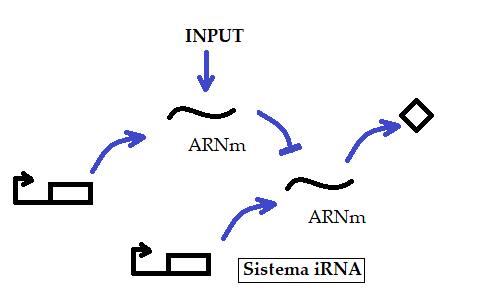
\includegraphics[scale=0.6]{iRNA}
\caption{iRNA system scheme.}
\label{fig:estructura}
\end{figure}


\begin{align*}
    M &\xrightarrow[]{\big{K_M}} M+1         & Z&\xrightarrow[]{\big{K_+EM}} Z+1              & T&\xrightarrow[]{\big{K_T}} T+1       & P&\xrightarrow[]{\big{K_PT}} P+1\\
    M &\xrightarrow[]{\big{K_-Z}} M+1        & Z&\xrightarrow[]{\big{\mu_-R}} Z+1             & T&\xrightarrow[]{\big{\mu_-R}} T+1    & P&\xrightarrow[]{\big{\gamma_PP}} P-1\\
    M &\xrightarrow[]{\big{K_+ME}} M-1       & Z&\xrightarrow[]{\big{\mu_+ZT}} Z-1            & T&\xrightarrow[]{\big{\mu_+ZT}} T-1   & R&\xrightarrow[]{\big{\mu_+ZT}} R+1\\
    M &\xrightarrow[]{\big{\gamma_MM}} M-1   & Z&\xrightarrow[]{\big{(\gamma_Z + K_-)Z}} Z-1  & T&\xrightarrow[]{\big{\gamma_TT}} T-1 & R&\xrightarrow[]{\big{(\gamma_R + \mu_-)R}} R-1
\end{align*}

\subsubsection{ Langevin equations}

Langevin equations derived for this system without the noise term.

\begin{align*}
    \frac{d}{dt}M &= K_M - \gamma_MM + K_-Z - K_+ME\\
    \frac{d}{dt}Z &= K_+EM + \mu_-R - (\gamma_Z + K_-)Z - \mu_+ZT\\
    \frac{d}{dt}T &= K_T + \mu_-R - \gamma_TT - \mu_+ZT\\
    \frac{d}{dt}P &= K_PT - \gamma_PP\\
    \frac{d}{dt}R &= \mu_+ZT - (\gamma_R + \mu_-)R
\end{align*}


\subsection{ Master equation}

Equation that describes the probability change over time, determined by the amount of particles in a certain state $(M, Z, T, P, R)$. Here the state is not always specified entirely. For example: $P(T-1)$ refers to the state $(M, Z, T, P, R)$ in which only the variable $T$ is changed by $-1$; $P(T-1)=P(M, Z, T-1, P, R)$.

\begin{align*}
    \frac{d}{dt}P(M, Z, T, P, R) &= K_MP(M-1) - K_MP(M) + \gamma_M(M+1)P(M+1) - \gamma_MMP(M)\\
                                 &+ K_-(Z+1)P(M-1,Z+1) - K_-ZP(M,Z)\\
                                 &+ K_+E(M+1)P(M+1,Z-1) - K_+EMP(M,Z)\\
                                 &+ \mu_-(R+1)P(Z-1,T-1,R+1) - \mu_-RP(Z,T,R)\\
                                 &+ \gamma_Z(Z+1)P(Z+1) - \gamma_ZZP(Z)\\
                                 &+ \mu_+(T+1)(Z+1)P(Z+1,T+1,R-1) - \mu_+ZTP(Z,T,R)\\
                                 &+ K_TP(T-1) - K_TP(T) + \gamma_T(T+1)P(T+1) - \gamma_TTP(T)\\
                                 &+ K_PTP(P-1) - K_PTP(P) + \gamma_P(P+1)P(P+1) - \gamma_PPP(P)\\
                                 &+ \gamma_R(R+1)P(R+1) - \gamma_RRP(R)
\end{align*}

Defining:
\\*
\begin{equation*}
    F = \sum_M\sum_Z\sum_T\sum_P\sum_R X_1^MX_2^ZX_3^TX_4^PX_5^RP(M,Z,T,P,R)
\end{equation*}


A system of associated variables is obtained:

\begin{align*}
    M &\xrightarrow{F} X_1 & Z&\xrightarrow{F} X_2 & T & \xrightarrow{F} X_3  &  P &\xrightarrow{F} X_4  &  R &\xrightarrow{F} X_5
\end{align*}

Then, applying the above definition to the master equation, the latter transforms into the moment-generating function of the $P(M,Z,T,P,R)$ distribution: 

\begin{equation}
    \left.\begin{aligned}
            \frac{d}{dt}F &= K_M(X_1-1) - \gamma_M(X_1-1)\frac{\partial}{\partial X_1} + K_-(X_1-X_2)\frac{\partial}{\partial X_2}\\
                          &+ K_+E(X_2-X_1)\frac{\partial}{\partial X_1} + \mu_-(X_2X_3-X_5)\frac{\partial}{\partial X_5} + \mu_+(X_5-X_2X_3)\frac{\partial}{\partial X_2}\frac{\partial}{\partial X_3}\\
                          &- \gamma_Z(X_2-1)\frac{\partial}{\partial X_2} + K_T(X_3-1) - \gamma_T(X_3-1)\frac{\partial}{\partial X_3}\\
                          &+ K_PX_3(X_4-1)\frac{\partial}{\partial X_3} - \gamma_P(X_4-1)\frac{\partial}{\partial X_4} - \gamma_R(X_5-1)\frac{\partial}{\partial X_5}
            \end{aligned}
    \right\}
    \qquad DF
 \end{equation}
\\*
\\*
Where $D$ is defined as the differential operator that satisfies: $\Dot{F} = DF$. Now, defining $\partial_i = \frac{\partial}{\partial X_i}$, the equations for the moments are generated via derivatives of $F$.

\begin{itemize}
    \item $\partial_1$
\end{itemize}
\begin{align*}
    \partial_1\Dot{F} &= K_MF - \gamma_M\partial_1F + K_-\partial_2F - K_+E\partial_1F + D\partial_1F\\
      \Longrightarrow & <\Dot{M}> = K_M - (\gamma_M+K_+E)<M> + K_-<Z>
\end{align*}

\begin{itemize}
    \item $\partial_2$
\end{itemize}
\begin{align*}
    \partial_2\Dot{F} &= -K_-\partial_2F + K_+E\partial_1F + \mu_-X_3\partial_5F - \mu_+X_3\partial_2\partial_3F - \gamma_z\partial_2F + D\partial_2F\\
    \Longrightarrow   &<\Dot{Z}> = K_+E<M> + \mu_-<R> - \mu_+<ZT> - (K_-+\gamma_Z)<Z>
\end{align*}

\begin{itemize}
    \item $\partial_3$
\end{itemize}
\begin{align*}
    \partial_3\Dot{F} &= \mu_-X_2\partial_5F - \mu_+X_2\partial_2\partial_3F + K_TF - \gamma_T\partial_3F + K_P(X_4-1)\partial_3F + D\partial_3F\\
    \Longrightarrow   & <\Dot{T}> = \mu_-<R> - \mu_+<ZT> + K_T - \gamma_T<T>
\end{align*}

\begin{itemize}
    \item $\partial_4$
\end{itemize}
\begin{align*}
    \partial_4\Dot{F} &= K_PX_3\partial_3F - \gamma_P\partial_4F + D\partial_4F\\
    \Longrightarrow   & <\Dot{P}> = K_P<T> - \gamma_P<P>
\end{align*}

\begin{itemize}
    \item $\partial_5$
\end{itemize}
\begin{align*}
    \partial_5\Dot{F} &= -\mu_-\partial_5F + \mu_+\partial_2\partial_3F - \gamma_R\partial_5F + D\partial_5F\\
    \Longrightarrow   & <\Dot{R}> = \mu_+<ZT> - (\mu_- + \gamma_R)<R>
\end{align*}

\begin{itemize}
    \item $\partial_1\partial_1$
\end{itemize}
\begin{align*}
    \partial_1\partial_1\Dot{F} &= 2[K_M\partial_1F - \gamma_M\partial_1\partial_1F + K_-\partial_1\partial_2F - K_+E\partial_1\partial_1F] + D\partial_1^2F\\
    \Longrightarrow             & <\Dot{M^2}> - <\Dot{M}> = 2\{K_M<M> - (\gamma_M + K_+E)[<M^2>-<M>] + K_-<MZ>\}
\end{align*}

\begin{itemize}
    \item $\partial_1\partial_2$
\end{itemize}
\begin{align*}
    \partial_1\partial_2\Dot{F} &= K_M\partial_2F - \gamma_M\partial_1\partial_2F + K_-\partial_2^2F - K_+E\partial_1\partial_2F - K_-\partial_1\partial_2F + K_+E\partial_1^2F\\
                                &+ \mu_-X_3\partial_1\partial_5F - \mu_+X_3\partial_1\partial_2\partial_3F - \gamma_Z\partial_1\partial_2F + D\partial_1\partial_2F\\
                \Longrightarrow & <\Dot{MZ}> = (K_M - K_-)<Z> + K_-<Z^2> + K_+E[<M^2>-<M>]\\
                                & \hspace{40pt}+ \mu_-<MR> - \mu_+<MZT> - (\gamma_M + \gamma_Z + K_- + K_+E)<MZ>
\end{align*}

\begin{itemize}
    \item $\partial_1\partial_3$
\end{itemize}
\begin{align*}
    \partial_1\partial_3\Dot{F} &= K_M\partial_3F - \gamma_M\partial_1\partial_3F + K_-\partial_2\partial_3F - K_+E\partial_1\partial_3F + \mu_-X_2\partial_1\partial_5F - \mu_+X_2\partial_1\partial_5F\\
                                &- \mu_+X_2\partial_1\partial_2\partial_3F + K_T\partial_1F - \gamma_T\partial_1\partial_3F + K_P(X_4-1)\partial_1\partial_3F + D\partial_1\partial_3F\\
            \Longrightarrow     & <\Dot{MT}> = K_M<T> - (\gamma_M + \gamma_T + K_+E)<MT> + K_-<ZT>\\
                                & \hspace{40pt}+ \mu_-<MR> + K_T<M> - \mu_+<MZT>
\end{align*}

\begin{itemize}
    \item $\partial_1\partial_4$
\end{itemize}
\begin{align*}
    \partial_1\partial_4\Dot{F} &= K_M\partial_4F - \gamma_M\partial_1\partial_4F + K_-\partial_2\partial_4F - K_+E\partial_1\partial_4F + K_PX_3\partial_1\partial_3F\\
                                &- \gamma_P\partial_1\partial_4F + D\partial_1\partial_4F\\
                \Longrightarrow & <\Dot{MP}> = K_M<P> - (\gamma_M + \gamma_P + K_+E)<MP> + K_-<ZP> + K_P<MT>
\end{align*}

\begin{itemize}
    \item $\partial_1\partial_5$
\end{itemize}
\begin{align*}
    \partial_1\partial_5\Dot{F} &= K_M\partial_5F - \gamma_M\partial_1\partial_5F + K_-\partial_2\partial_5F - K_+E\partial_1\partial_5F\\
                                &- \mu_-\partial_1\partial_5F + \mu_+\partial_1\partial_2\partial_3F - \gamma_R\partial_1\partial_5F + D\partial_1\partial_5F\\
            \Longrightarrow     & <\Dot{MR}> = K_M<R> + K_-<ZR> + \mu_+<MZT>\\
                                &\hspace{40pt}- (\gamma_M + \gamma_R + \mu_- + K_+E)<MR>
\end{align*}

\begin{itemize}
    \item $\partial_2\partial_2$
\end{itemize}
\begin{align*}
    \partial_2\partial_2\Dot{F} &= 2[-K_-\partial_2^2F + K_+E\partial_1\partial_2F + \mu_-X_3\partial_2\partial_5F - \mu_+X_3\partial_2^2\partial_3F - \gamma_Z\partial_2^2F + D\partial_2^2F]\\
    \Longrightarrow & <\Dot{Z^2}> - <\Dot{Z}> = 2\{-(K_- + \gamma_Z)[<Z^2>-<Z>] + K_+E<MZ> \\
    &\hspace{80pt}+ \mu_-<ZR> - \mu_+[<Z^2T> - <ZT>]\}
\end{align*}

\begin{itemize}
    \item $\partial_2\partial_3$
\end{itemize}
\begin{align*}
    \partial_2\partial_3\Dot{F} &= -K_-\partial_2\partial_3F + K_+E\partial_1\partial_3 + \mu_-\partial_5F + \mu_-X_3\partial_3\partial_5F - \mu_+\partial_2\partial_3F\\
                                &- \mu_+X_3\partial_2\partial_3^2F - \gamma_Z\partial_2\partial_3F + \mu_-X_2\partial_2\partial_5F - \mu_+X_2\partial_2^2\partial_3F\\
                                &+ K_T\partial_2F - \gamma_T\partial_2\partial_3F + K_P(X_4-1)\partial_2\partial_3F + D\partial_2\partial_3F\\
            \Longrightarrow     &<\Dot{ZT}> = K_T<Z> - (K_- + \cancel{\mu_+} + \gamma_Z + \gamma_T)<ZT> + K_+E<MT> \\
                                & \hspace{40pt} + \mu_-<R> + \mu_-<TR> - \mu_+[<ZT^2>-\cancel{<ZT>}]\\
                                & \hspace{40pt} + \mu_-<ZR> - \mu_+[<Z^2T>-<ZT>]
\end{align*}

\begin{itemize}
    \item $\partial_2\partial_4$
\end{itemize}
\begin{align*}
    \partial_2\partial_4\Dot{F} &= -K_-\partial_2\partial_4F + K_+E\partial_1\partial_4F + \mu_-X_3\partial_4\partial_5F - \mu_+X_3\partial_2\partial_3\partial_4F\\
                                &- \gamma_Z\partial_2\partial_4F + K_PX_3\partial_2\partial_3F - \gamma_P\partial_2\partial_4F + D\partial_2\partial_4F\\
                \Longrightarrow & <\Dot{ZP}> = -(K_- + \gamma_Z + \gamma_P)<ZP> + K_+E<MP> + \mu_-<PR>\\
                                & \hspace{40pt} - \mu_+<ZTP> + K_P<ZT>
\end{align*}

\begin{itemize}
    \item $\partial_2\partial_5$
\end{itemize}
\begin{align*}
    \partial_2\partial_5\Dot{F} &= -K_-\partial_2\partial_5F + K_+E\partial_1\partial_5F + \mu_-X_3\partial_5^2F - \mu_+X_3\partial_2\partial_3\partial_5F\\
                                &- \gamma_Z\partial_2\partial_5F - \mu_-\partial_2\partial_5F + \mu_+\partial_2^2\partial_3F - \gamma_R\partial_2\partial_5F + D\partial_2\partial_5F\\
            \Longrightarrow     &<\Dot{ZR}> = - (K_- + \mu_- + \gamma_Z + \gamma_R)<ZR> + K_+E<MR> \\
                                & \hspace{40pt} + \mu_-[<R^2>-<R>] -\mu_+<ZTR> + \mu_+[<Z^2T>-<ZT>]
\end{align*}

\begin{itemize}
    \item $\partial_3\partial_3$
\end{itemize}
\begin{align*}
    \partial_3\partial_3\Dot{F} &= 2[\mu_-X_2\partial_3\partial_5F - \mu_+X_2\partial_2\partial_3^2F + K_T\partial_3F - \gamma_T\partial_3^2 + K_P(X_4-1)\partial_3^2F + D\partial_3^2F]\\
    \Longrightarrow & <\Dot{T^2}>-<\Dot{T}> = 2\{\mu_-<TR> - \mu_+[<ZT^2> - <ZT>]\\
                    & \hspace{80pt}+ K_T<T> - \gamma_T[<T^2>-<T>]\}
\end{align*}

\begin{itemize}
    \item $\partial_3\partial_4$
\end{itemize}
\begin{align*}
    \partial_3\partial_4\Dot{F} &= \mu_-X_2\partial_4\partial_5F - \mu_+X_2\partial_2\partial_3\partial_4F + K_T\partial_4F - \gamma_T\partial_3\partial_4F + K_P\partial_3F\\
                                &+ K_P(X_4-1)\partial_3\partial_4F + K_PX_3\partial_3^2F - \gamma_P\partial_3\partial_4F + D\partial_3\partial_4F\\
                \Longrightarrow & <\Dot{TP}> = -(\gamma_T + \gamma_P)<TP> + \mu_-<PR> - \mu_+<ZTP> + K_T<P>\\
                                & \hspace{40pt}+ \cancel{K_P<T>} + K_P[<T^2>-\cancel{<T>}]
\end{align*}

\begin{itemize}
    \item $\partial_3\partial_5$
\end{itemize}
\begin{align*}
    \partial_3\partial_5\Dot{F} &= \mu_-X_2\partial_5^2F - \mu_+X_2\partial_2\partial_3\partial_5F + K_T\partial_5F - \gamma_T\partial_3\partial_5F\\
                                & + K_P(X_4-1)\partial_3\partial_5F - \mu_-\partial_3\partial_5F + \mu_+\partial_2\partial_3^2F - \gamma_R\partial_3\partial_5F + D\partial_3\partial_5F\\
                \Longrightarrow & <\Dot{TR}> = -(\gamma_T + \gamma_R + \mu_-)<TR> + K_T<R> - \mu_+<ZTR>\\
                                & \hspace{40pt} + \mu_-[<R^2>-<R>] + \mu_+[<ZT^2>-<ZT>]
\end{align*}

\begin{itemize}
    \item $\partial_4\partial_4$
\end{itemize}
\begin{align*}
    \partial_4\partial_4\Dot{F} &= 2[K_PX_3\partial_3\partial_4 - \gamma_P\partial_4^2F] + D\partial_4^2F\\
    \Longrightarrow & <\Dot{P^2}>-<\Dot{P}> = 2\{K_P<TP> - \gamma_P[<P^2>-<P>]\}
\end{align*}

\begin{itemize}
    \item $\partial_4\partial_5$
\end{itemize}
\begin{align*}
    \partial_4\partial_5\Dot{F} &= K_PX_3\partial_3\partial_5F - \gamma_P\partial_4\partial_5F - \mu_-\partial_4\partial_5F + \mu_+\partial_2\partial_3\partial_4F\\
                                &- \gamma_R\partial_4\partial_5F + D\partial_4\partial_5F\\
                \Longrightarrow & <\Dot{PR}> = K_P<TR> - (\gamma_P + \gamma_R+\mu_-)<PR> + \mu_+<ZTP>
\end{align*}

\begin{itemize}
    \item $\partial_5\partial_5$
\end{itemize}
\begin{align*}
    \partial_5\partial_5\Dot{F} &= 2[-\mu_-\partial_5^2F + \mu_+\partial_2\partial_3\partial_5F - \gamma_R\partial_5^2F] + D\partial_5^2F\\
            \Longrightarrow     & <\Dot{R^2}> - <\Dot{R}> = 2\{-(\gamma_R+ \mu_-)[<R^2> -<R>] + \mu_+<ZTR>\}
\end{align*}
\\*
\\*
Assuming steady state (all time derivatives equal to zero) and using equations $\partial_i$ for $i\in\{1,2,3,4,5\}$ it can be proven that the expected value of $M, Z, T, P, R$ can be written in terms of $<ZT>$. This happens because equations $\partial_i$ yield a linear system which has six variables and only five equations. Taking into account the other 15 equations, the total system would be one of 25 variables and only 20 equations. In order to construct $\eta_P^2$ for this system, only 2 of all those variables are needed: $<P^2>$ and $<ZT>$.
























\end{document}
